%
% section 3.3.2
%
\setcounter{subsection}{1}
\subsection{Το Πρωτόκολλο Δυναμικής Διευθέτησης Υπολογιστή DHCP}

Το DHCP λειτουργεί με παρόμοιο τρόπο με το BOOTP και επεκτείνει τη λειτουργία του. Πρόκειται για πρωτόκολλο που χρησιμοποιεί το μοντέλο \emph{πελάτη -- εξυπηρετητή} και εκτελείται στο επίπεδο εφαρμογής. Το DHCP χρησιμοποιεί πακέτα UDP και έχει καθορισμένες θύρες τόσο για τον εξυπηρετητή (θύρα 67) όσο και για τον πελάτη (θύρα 68).

Το DHCP μας επιτρέπει να στείλουμε σε ένα μόνο  μήνυμα ένα πλήθος ρυθμίσεων και όχι μόνο μια διεύθυνση όπως το RARP. Τυπικά στέλνουμε ρυθμίσεις όπως τη διεύθυνση, τη μάσκα δικτύου, την προεπιλεγμένη πύλη (δρομολογητή) και έναν ή περισσότερους εξυπηρετητές DNS. Το DHCP καθορίζει τρεις τύπους εκχώρησης διευθύνσεων:

\begin{itemize}
\item \textbf{Τη μη αυτόματη (ή χειροκίνητη) ρύθμιση (manual configuration):} Στην περίπτωση αυτή ο διαχειριστής ορίζει συγκεκριμένες διευθύνσεις που θα πάρουν συγκεκριμένοι υπολογιστές και ο εξυπηρετητής απλά στέλνει πάντα τις ίδιες αυτές ρυθμίσεις στα συγκεκριμένα μηχανήματα.
\item \textbf{Την αυτόματη ρύθμιση (automatic configuration):} Σε αυτή ο εξυπηρετητής DHCP στέλνει μια μόνιμη διεύθυνση σε ένα υπολογιστή ο οποίος συνδέεται για πρώτη φορά.
\item \textbf{Τη δυναμική ρύθμιση (dynamic configuration):} Σε αυτή ο εξυπηρετητής DHCP δανείζει (μισθώνει) μια διεύθυνση σε ένα υπολογιστή για κάποιο περιορισμένο χρονικό διάστημα.
\end{itemize}

Η δυναμική ρύθμιση είναι η πιο συχνά χρησιμοποιούμενη.

\begin{inthebox}
\textbf{Ποια η διαφορά μεταξύ αυτόματης και μη αυτόματης ρύθμισης; Αφού και οι δυο στέλνουν μόνιμες διευθύνσεις.}

Στην αυτόματη ρύθμιση, αποδίδεται στον υπολογιστή μια μόνιμη διεύθυνση από μια λίστα διαθέσιμων διευθύνσεων που διατηρεί ο εξυπηρετητής. Στη χειροκίνητη ρύθμιση, η μόνιμη διεύθυνση επιλέγεται απευθείας από τον διαχειριστή. Είναι σημαντικό για ορισμένα κρίσιμα μηχανήματα σε ένα δίκτυο να έχουν πάντοτε την ίδια και γνωστή σε μας διεύθυνση, ώστε να μπορούμε να συνδεθούμε σε αυτά χρησιμοποιώντας το IP τους ακόμα και όταν για κάποιο λόγο δεν λειτουργούν υπηρεσίες ονομάτων όπως το DNS που θα δούμε παρακάτω.\\
\end{inthebox}

\emph{Πλεονεκτήματα του DHCP:} Βασικό πλεονέκτημα του DHCP από τη σκοπιά των απλών (μη-τεχνικών) χρηστών είναι η απλούστευση στη σύνδεση σε ένα δίκτυο. Οι περισσότεροι χρήστες δεν κατανοούν την τεχνική πολυπλοκότητα της σύνδεσης σε ένα δίκτυο και το DHCP τους δίνει τη δυνατότητα να συνδεθούν εύκολα σε αυτό. Ταυτόχρονα διευκολύνεται και η εργασία του διαχειριστή που δεν χρειάζεται πλέον να κάνει σε κάθε μηχάνημα χωριστά ρυθμίσεις, αλλά μπορεί να τις διαχειρίζεται κεντρικά και να συντηρεί ευκολότερα το δίκτυο. 

Εκτός από τις ρυθμίσεις που αναφέραμε παραπάνω, το πρωτόκολλο DHCP μπορεί να στείλει στον υπολογιστή ή σε κάθε του δικτυακή σύνδεση ρυθμίσεις για το επίπεδο ζεύξης δεδομένων, για το πρωτόκολλο TCP (επίπεδο μεταφοράς), καθώς και για υπηρεσίες (επίπεδο εφαρμογής) όπως για παράδειγμα διακομιστές χρόνου (NTP, χρησιμοποιούνται για την αυτόματη ρύθμιση της ώρας στους υπολογιστές), διακομιστές αλληλογραφίας κλπ. Οι ρυθμίσεις αυτές περιγράφονται στο \href{https://www.ietf.org/rfc/rfc2132.txt}{RFC2132} και τα συμπληρωματικά του.

\begin{figure}[!ht]
 \centering
 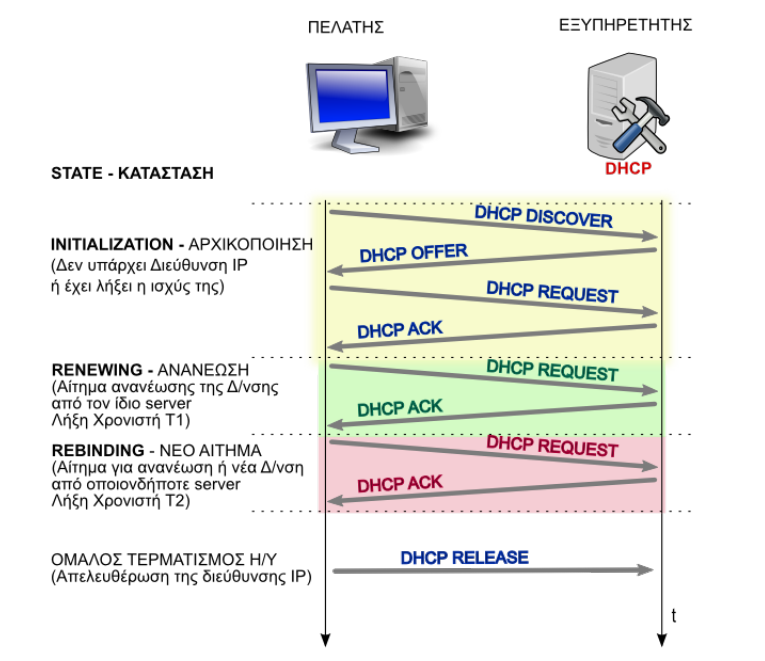
\includegraphics[width=0.85\textwidth]{images/chapter3/3-18}
 \caption {\textsl{Η Λειτουργία του DHCP}}
 \label{3-18}
\end{figure}

Ένας υπολογιστής -- πελάτης που έχει ρυθμιστεί να χρησιμοποιεί την υπηρεσία DHCP, αμέσως μετά την εκκίνηση του, εκτελεί τα παρακάτω βήματα (σχήμα \ref{3-18}):

\begin{itemize}
\item Δημιουργεί ένα αυτοδύναμο πακέτο \textbf{UDP DHCPDISCOVER} από τη θύρα 68 στην θύρα προορισμού 67. Όλη η επικοινωνία του πρωτοκόλλου DHCP (εφαρμογής) ενθυλακώνεται σε πρωτόκολλο UDP (μεταφοράς).
\item Το πακέτο UDP το ενθυλακώνει σε πακέτο IP στο επίπεδο δικτύου. Δεδομένου ότι ο υπολογιστής μας δεν διαθέτει διεύθυνση δικτύου, χρησιμοποιείται ως διεύθυνση αποστολέα η ειδική διεύθυνση 0.0.0.0. Ο υπολογιστής δεν γνωρίζει την διεύθυνση IP του εξυπηρετητή DHCP, οπότε ως διεύθυνση παραλήπτη χρησιμοποιείται η διεύθυνση εκπομπής 255.255.255.255.
\item Το παραπάνω πακέτο IP ενθυλακώνεται σε ένα πλαίσιο στο επίπεδο ζεύξης δεδομένων. Η φυσική διεύθυνση προέλευσης (48 bit) είναι η πραγματική του αποστολέα. Καθώς δεν γνωρίζουμε τη φυσική διεύθυνση του εξυπηρετητή DHCP, χρησιμοποιείται η διεύθυνση εκπομπής FF:FF:FF:FF:FF:FF. Το πλαίσιο στέλνεται στο τοπικό δίκτυο. 
\item Αν υπάρχουν εξυπηρετητές DHCP ανταποκρίνονται  ο καθένας με ένα πακέτο \textbf{DHCPOFFER} το οποίο απευθύνεται στη θύρα 68 και ενθυλακώνεται σε ένα πακέτο IP εκπομπής (255.255.255.255) το οποίο με τη σειρά του ενθυλακώνεται σε ένα πλαίσιο εκπομπής (FF:FF:FF:FF:FF:FF).  Καθώς οι διακομιστές γνωρίζουν από το πακέτο DHCPDISCOVER τη φυσική διεύθυνση του αποστολέα, μπορούν να απαντήσουν με πλαίσιο που να απευθύνεται απευθείας σε αυτόν και όχι με πλαίσιο εκπομπής. Το πακέτο DHCPOFFER περιέχει όλες τις απαιτούμενες ρυθμίσεις δικτύου.
\item  Ο υπολογιστής -- πελάτης επιλέγει τις ρυθμίσεις που επιθυμεί από ένα από τους εξυπηρετητές που απάντησαν (οι υπόλοιποι ενημερώνονται και αποσύρουν τις προσφορές τους) και το δηλώνει αποστέλλοντας ένα πακέτο\\ \textbf{DHCPREQUEST} στο οποίο ζητά τις προσφερόμενες ρυθμίσεις.
\item Ο εξυπηρετητής DHCP που προσέφερε τις ρυθμίσεις επιβεβαιώνει την προσφορά του με ένα πακέτο \textbf{DHCPACK} (επιβεβαίωσης).
\end{itemize}

Μετά τη λήψη της επιβεβαίωσης DHCPACK ο υπολογιστής πλέον λειτουργεί με τις ρυθμίσεις δικτύου που πήρε μέσω του πακέτου DHCPOFFER. Στην κατάσταση αυτή ο υπολογιστής ονομάζεται δεσμευμένος (BOUND). Στη συνηθισμένη δυναμική ρύθμιση, η διεύθυνση IP παραχωρείται στον υπολογιστή για συγκεκριμένο χρονικό διάστημα, χαρακτηρίζεται δε ως \emph{μίσθωση, lease}. Το χρονικό αυτό διάστημα μπορεί να ρυθμιστεί από το διαχειριστή στις ρυθμίσεις του εξυπηρετητή DHCP.

Από τη στιγμή αυτή, αρχίζει η σχετική μέτρηση χρόνου: πριν λήξει ο χρόνος μίσθωσης, ο υπολογιστής θα προβεί σε ενέργειες για την ανανέωση ή παράταση της. Ο υπολογιστής κρατά δύο χρόνους:

\begin{itemize}
\item Το χρόνο Τ1 -- τυπικά 0.5 * χρόνος μίσθωσης -- μετά τον οποίο προσπαθεί να ανανεώσει τη μίσθωση από το διακομιστή ο οποίος έδωσε αρχικά τη διεύθυνση. Σε αυτή την περίπτωση λέμε ότι ο υπολογιστής βρίσκεται σε κατάσταση \emph{RENEWING (ανανέωσης)}. Για την διαδικασία αυτή στέλνει εκ νέου πακέτο DHCPREQUEST - unicast δηλ. προς το συγκεκριμένο διακομιστή (δεν χρησιμοποιεί διεύθυνση εκπομπής). 
\item το χρόνο Τ2 -- τυπικά 0.875 * χρόνος μίσθωσης -- μετά τον οποίο αναζητά ανανέωση ή νέα διεύθυνση από οποιοδήποτε πλέον διακομιστή DHCP του δικτύου. Σε αυτή την περίπτωση ο υπολογιστής είναι σε κατάσταση \emph{REBINDING}. Για τη διαδικασία αυτή στέλνει πακέτο DHCPREQUEST - broadcast χρησιμοποιεί δηλ. διεύθυνση εκπομπής. 
\end{itemize}

Ο χρόνος Τ1 είναι προφανώς μικρότερος του T2.

Όταν ο υπολογιστής τερματίζει τη λειτουργία του ομαλά και πριν λήξει η μίσθωση της διεύθυνσης, ζητά την απελευθέρωση της (ώστε να μπορεί να δοθεί σε άλλον υπολογιστή αν υπάρχει ανάγκη) στέλνοντας πριν το τερματισμό ένα πακέτο\\ \textbf{DHCPRELEASE} στο διακομιστή DHCP.

Στο πρωτόκολλο DHCP προβλέπονται ακόμα τα εξής μηνύματα:

\begin{itemize}
\item \textbf{DHCPNAK:} Από το διακομιστή προς τον πελάτη: Αν μετά από το\\ DHCPREQUEST, ο διακομιστής δεν επιβαιώσει ως σωστές τις ρυθμίσεις που ζητά ο πελάτης, απαντά με ένα μήνυμα μη-επιβεβαίωσης DHCPNAK.
\item \textbf{DHCPDECLINE:} Από τον πελάτη προς το διακομιστή: Αν μετά τη λήψη μιας προσφοράς μέσω DHCPOFFER ο πελάτης διαπιστώσει ότι οι ρυθμίσεις που του στάλθηκαν είναι σε σύγκρουση με άλλο υπολογιστή στο δίκτυο, απορρίπτει την προσφορά στέλνοντας ένα πακέτο DHCPDECLINE. Έπειτα ξεκινά τη διαδικασία από την αρχή στέλνοντας πακέτο DHCPDISCOVER.
\item \textbf{DHCPINFORM:} Αν μετά την αρχική λήψη ρυθμίσεων μέσω DHCPOFFER ο πελάτης χρειάζεται επιπλέον ρυθμίσεις δικτύου, δεν μπορεί να χρησιμοποιήσει ξανά το πακέτο DHCPREQUEST. Στην περίπτωση αυτή τις ζητά με ένα αίτημα DHCPINFORM. 
\end{itemize}

Η λειτουργία του DHCP υποστηρίζεται και από \textbf{Πράκτορες Αναμετάδοσης, DHCP Relay Agents}.  Ένας υπολογιστής πελάτης που βρίσκεται σε διαφορετικό τμήμα ή φυσικό δίκτυο από αυτό που βρίσκεται ο διακομιστής DHCP δεν μπορεί να επικοινωνήσει απευθείας με αυτόν καθώς δεν διαθέτει διεύθυνση IP (οι φυσικές διευθύνσεις ισχύουν μόνο στο συγκεκριμένο τμήμα δικτύου και δεν μπορούν να δρομολογηθούν). Ένας υπολογιστής που βρίσκεται στο ίδιο φυσικό δίκτυο με τον πελάτη μπορεί να λειτουργήσει ως αναμεταδότης, προωθώντας τα μηνύματα του πελάτη προς το διακομιστή DHCP στο άλλο δίκτυο και επιστρέφοντας τις απαντήσεις του.

Το πρωτόκολλο DHCP προτάθηκε ως επέκταση του BOOTP, αρχικά στα \href{https://www.ietf.org/rfc/rfc1531.txt}{RFC1531}, \href{https://www.ietf.org/rfc/rfc1541.txt}{RFC1541} τα οποία αντικαταστάθηκαν από το \href{https://www.ietf.org/rfc/rfc2131.txt}{RFC2131}. Σε αυτό και τα συμπληρωματικά του βρίσκονται όλες οι απαιτούμενες πληροφορίες για τη λειτουργία του.



